\documentclass[conference]{IEEEtran}
\IEEEoverridecommandlockouts
% The preceding line is only needed to identify funding in the first footnote. If that is unneeded, please comment it out.
%\usepackage{cite}
\usepackage{amsmath,amssymb,amsfonts}
\usepackage{algorithmic}
\usepackage{enumitem}
\usepackage{algorithm}
\usepackage{graphicx}
\usepackage{textcomp}
\usepackage{titlesec}
\usepackage{tikz}
\usepackage{listings}
\usepackage[margin=0.3in]{geometry}
\usepackage{xcolor}
\def\BibTeX{{\rm B\kern-.05em{\sc i\kern-.025em b}\kern-.08em
    T\kern-.1667em\lower.7ex\hbox{E}\kern-.125emX}}
    
%\titleformat{\section}{\small}{}{1em}{}
%\titleformat{\subsection}{\scriptsize}{}{1em}{}
%\titleformat{\subsubsection}{\scriptsize}{}{1em}{}

\usepackage{listings}
\usepackage{color}

\definecolor{codegreen}{rgb}{0,0.6,0}
\definecolor{codegray}{rgb}{0.5,0.5,0.5}
\definecolor{codepurple}{rgb}{0.58,0,0.82}
\definecolor{backcolour}{rgb}{0.95,0.95,0.92}


\lstdefinestyle{mystyle}{
    commentstyle=\color{codegreen},
    numberstyle=\tiny\color{codegray},
    stringstyle=\color{codepurple},
    basicstyle=\ttfamily\footnotesize,
    breakatwhitespace=false,         
    breaklines=true,                 
    captionpos=b,                    
    keepspaces=true,                 
    numbers=left,                    
    numbersep=5pt,                  
    showspaces=false,                
    showstringspaces=false,
    showtabs=false,                  
    tabsize=2
}

\lstset{style=mystyle}


\begin{document}
\scriptsize 


\vspace{-0.3cm}
\subsection*{Functional Dependency and Closure}
\vspace{-0.1cm}

\noindent
Functional Dependency (FD) is like a rule that says one piece of data (like a person's name) can tell you another piece of data (like their birthdate). If you know the rule applies consistently, then you know the birthdate for each name without fail.

\vspace{-0.3cm}
\subsection*{Closure Set \( F+ \)}
\vspace{-0.1cm}

\noindent
The closure \( F+ \) is like knowing all the possible things you can find out if you know a starting piece of information under the rules of FD. For example, if knowing someone's name tells you their birthdate, and knowing their birthdate tells you their astrological sign, then knowing a name ultimately tells you both birthdate and astrological sign—that's the closure.

\noindent
\textbf{Example:} If you have a functional dependency:
\[ \text{Name} \rightarrow \text{Birthdate} \]
and another:
\[ \text{Birthdate} \rightarrow \text{Astrological Sign} \]
Then the closure of Name would be:
\[ \text{Name}+ = \{ \text{Name, Birthdate, Astrological Sign} \} \]

\vspace{-0.6cm}
\subsection*{Achieving Boyce-Codd Normal Form (BCNF)}
\vspace{-0.1cm}

\noindent
BCNF is like organizing your closet so that every item has one and only one place where it belongs. A database is in BCNF if every piece of data can be uniquely identified by a 'key' (like a label for a shelf in your closet), and there's no confusion about where to find data or how it links to other data.

\vspace{-0.3cm}
\subsection*{Relation Decomposition}
\vspace{-0.1cm}

\noindent
To get a database into BCNF, you might need to 'decompose' it, which means breaking it into smaller, well-organized parts. It's like deciding to separate your socks, shirts, and pants into different drawers instead of having them all in one place.

\noindent
\textbf{Example:} Suppose you have a table with courses and instructors, where the course code determines the instructor, and each instructor works in one department. This creates redundancy because the department can be determined by the course code.

\[ \text{Course Code} \rightarrow \text{Instructor} \]
\[ \text{Instructor} \rightarrow \text{Department} \]

To decompose into BCNF, you create separate tables:
\begin{itemize}
    \item One for courses and instructors, where course code is a unique identifier.
    \item Another for instructors and departments, where instructor is a unique identifier.
\end{itemize}

This way, each piece of information is found in only one place, and your data is well-organized.




\section*{Relational Algebra Operations}

\vspace{-0.1cm}

\begin{center}
\noindent
\textit{Students Table:} ID, Name, Age, Major. \\
\textit{Courses Table:} CourseID, Name, Credits.
\end{center}


\vspace{-0.7cm}
\subsection*{Basic Operations}
\vspace{-0.1cm}

\begin{itemize}[noitemsep,leftmargin=*]
\leftskip-\dimexpr\leftmargin %%%

% Select
\item[]{\textbf{Select} $(\sigma)$:
$\sigma_{\text{Age} > 21}(\text{Students})$. \\
Selects rows where age larger than 21 years.}

% Project
\item[]{\textbf{Project} $(\pi)$:
$\pi_{\text{Name, Major}}(\text{Students})$. \\
Selects the `Name` and `Major` columns from the `Students` table.}

% Union
\item[]{\textbf{Union} $(\cup)$:
$\pi_{\text{Name}}(\text{Students}) \cup \pi_{\text{Name}}(\text{Courses})$. \\
Combines the `Name` columns from `Students` and `Courses` tables.}

% Set Difference
\item[]{\textbf{Set Difference} $(-)$:
$\pi_{\text{Name}}(\text{Students}) - \pi_{\text{Name}}(\text{Courses})$. \\
Rows in the first relation (Students) but not in the second (Courses).}

% Cartesian Product
\item[]{\textbf{Cartesian Product} $(\times)$:
$\text{Students}_1 \times \text{Courses}_2$. \\
Creates pairs of every student with every course. Every $item_1$ goes with every $item_2$.}

% Rename
\item[]{\textbf{Rename} $(\rho)$:
$\rho_{\text{Pupils}(\text{ID, StudentName, StudentAge, Major})}(\text{Students})$. \\
Renames the `Students` table to `Pupils` and its attributes accordingly.}

% Intersection
\item[]{\textbf{Intersection} $(\cap)$:
$\pi_{\text{Name}}(\text{Students}) \cap \pi_{\text{Name}}(\text{Courses})$. \\
Finds names common to both `Students` and `Courses`.}

% Natural Join
\item[]{\textbf{Natural Join} $(\bowtie)$:
$\text{Students} \bowtie \text{Enrollments}$. \\
Joins `Students` and `Enrollments` on common attributes/columns.}

% Theta Join
\item[]{\textbf{Theta Join}:
$\text{Students} \bowtie_{\text{Students.Major = Courses.Name}} \text{Courses}$. \\
Joins `Students` and `Courses` where the student's major matches the course name.}

% Division
\item[]{\textbf{Division}:
$\text{Enrollments} \div \pi_{\text{CourseID}}(\sigma_{\text{Instructor = 'Dr. Smith'}}(\text{Courses}))$. \\
Finds students who are enrolled in all courses taught by 'Dr. Smith'.}


\item[]{\textbf{Projection, Join, Selection}: \\
$\pi_{\text{StudentName, CourseName}} (\sigma_{\text{Age} > 21} (\text{Students} \bowtie \text{Enrollments} \bowtie \text{Courses}))$ \\
Retrieves names of students older than 21 and their course names.}

\item[]{\textbf{Union and Intersection}: \\
\vspace{-0.2cm}
\begin{center}
$\left( \pi_{\text{Name}} (\sigma_{\text{Major} = 'CS'}(\text{Students})) \cup \pi_{\text{Name}} (\sigma_{\text{Age} > 21}(\text{Students})) \right) -  \left( \pi_{\text{Name}} (\sigma_{\text{Major} = 'CS'}(\text{Students})) \cap \pi_{\text{Name}} (\sigma_{\text{Age} > 21}(\text{Students})) \right)$ \\
\end{center}
Finds students either majoring in CS or older than 21, excluding those who meet both criteria.}

\item[]{\textbf{Nested Operations}: \\
$\pi_{\text{InstructorName}} (\sigma_{\text{CourseName} = 'Math'}(\text{Courses})) - \pi_{\text{InstructorName}} (\sigma_{\text{CourseName} = 'Physics'}(\text{Courses}))$ \\
Identifies instructors teaching 'Math' but not 'Physics'.}

\end{itemize}

\vspace{-0.3cm}
\section*{Logical Model}

\vspace{-0.1cm}

\noindent
Entity-Relationship (ER) Models visually represent relational databases, showing entities (real-world items), attributes (entity properties), and relationships (entity connections).

\vspace{-0.3cm}
\subsection*{Components}
\vspace{-0.1cm}

\begin{itemize}[noitemsep,leftmargin=*]
\leftskip-\dimexpr\leftmargin %%%
\item[] \textbf{Entity:} Represents real-world items. E.g., `Student`, `Course`.
\item[] \textbf{Attribute:} Entity properties. E.g., `Student` has `Name`, `Age`, `Major`.
\item[] \textbf{Relationship:} Connection between entities. E.g., `Enrollment` links `Student` and `Course`.
\end{itemize}

\vspace{-0.3cm}
\subsection*{Entity Types}
\vspace{-0.1cm}

\begin{itemize}[noitemsep,leftmargin=*]
\leftskip-\dimexpr\leftmargin %%%
\item[] \textbf{Strong Entity:} Exists independently. E.g., `Student`.
\item[] \textbf{Weak Entity:} Depends on another entity. E.g., `Classroom` depends on `School`.
\end{itemize}

\vspace{-0.3cm}
\subsection*{Attribute Types}
\vspace{-0.1cm}

\begin{itemize}[noitemsep,leftmargin=*]
\leftskip-\dimexpr\leftmargin %%%
\item[] \textbf{Simple Attribute:} Indivisible. E.g., `Name`.
\item[] \textbf{Composite Attribute:} Divisible into sub-parts. E.g., `Address` includes `Street`, `City`, `Zip`.
\item[] \textbf{Derived Attribute:} Calculated from other attributes. E.g., `Age` from `Date of Birth`.
\end{itemize}

\vspace{-0.3cm}
\noindent
\subsection*{Relationship Types}
\vspace{-0.1cm}

\begin{itemize}[noitemsep,leftmargin=*]
\leftskip-\dimexpr\leftmargin %%%
\item[] \textbf{Unary:} Within a single entity type. E.g., `Employee` supervises `Employee`.
\item[] \textbf{Binary:} Between two entity types. E.g., `Student` enrolls in `Course`.
\item[] \textbf{Ternary:} Among three entities. E.g., `Supplier` supplies `Part` to `Project`.
\end{itemize}

\vspace{-0.3cm}
\subsection*{Cardinality Constraints}
\vspace{-0.1cm}

\begin{itemize}[noitemsep,leftmargin=*]
\leftskip-\dimexpr\leftmargin %%%
\item[] \textbf{One-to-One:} Single relation each way. E.g., `Person` to `Passport`.
\item[] \textbf{One-to-Many:} One to multiple relations. E.g., `Instructor` teaches multiple `Courses`.
\item[] \textbf{Many-to-Many:} Multiple relations each way. E.g., `Students` enrolling in `Courses`.
\end{itemize}
\vspace{-0.3cm}
\subsection*{Tables and Keys}
\vspace{-0.1cm}

\begin{center}
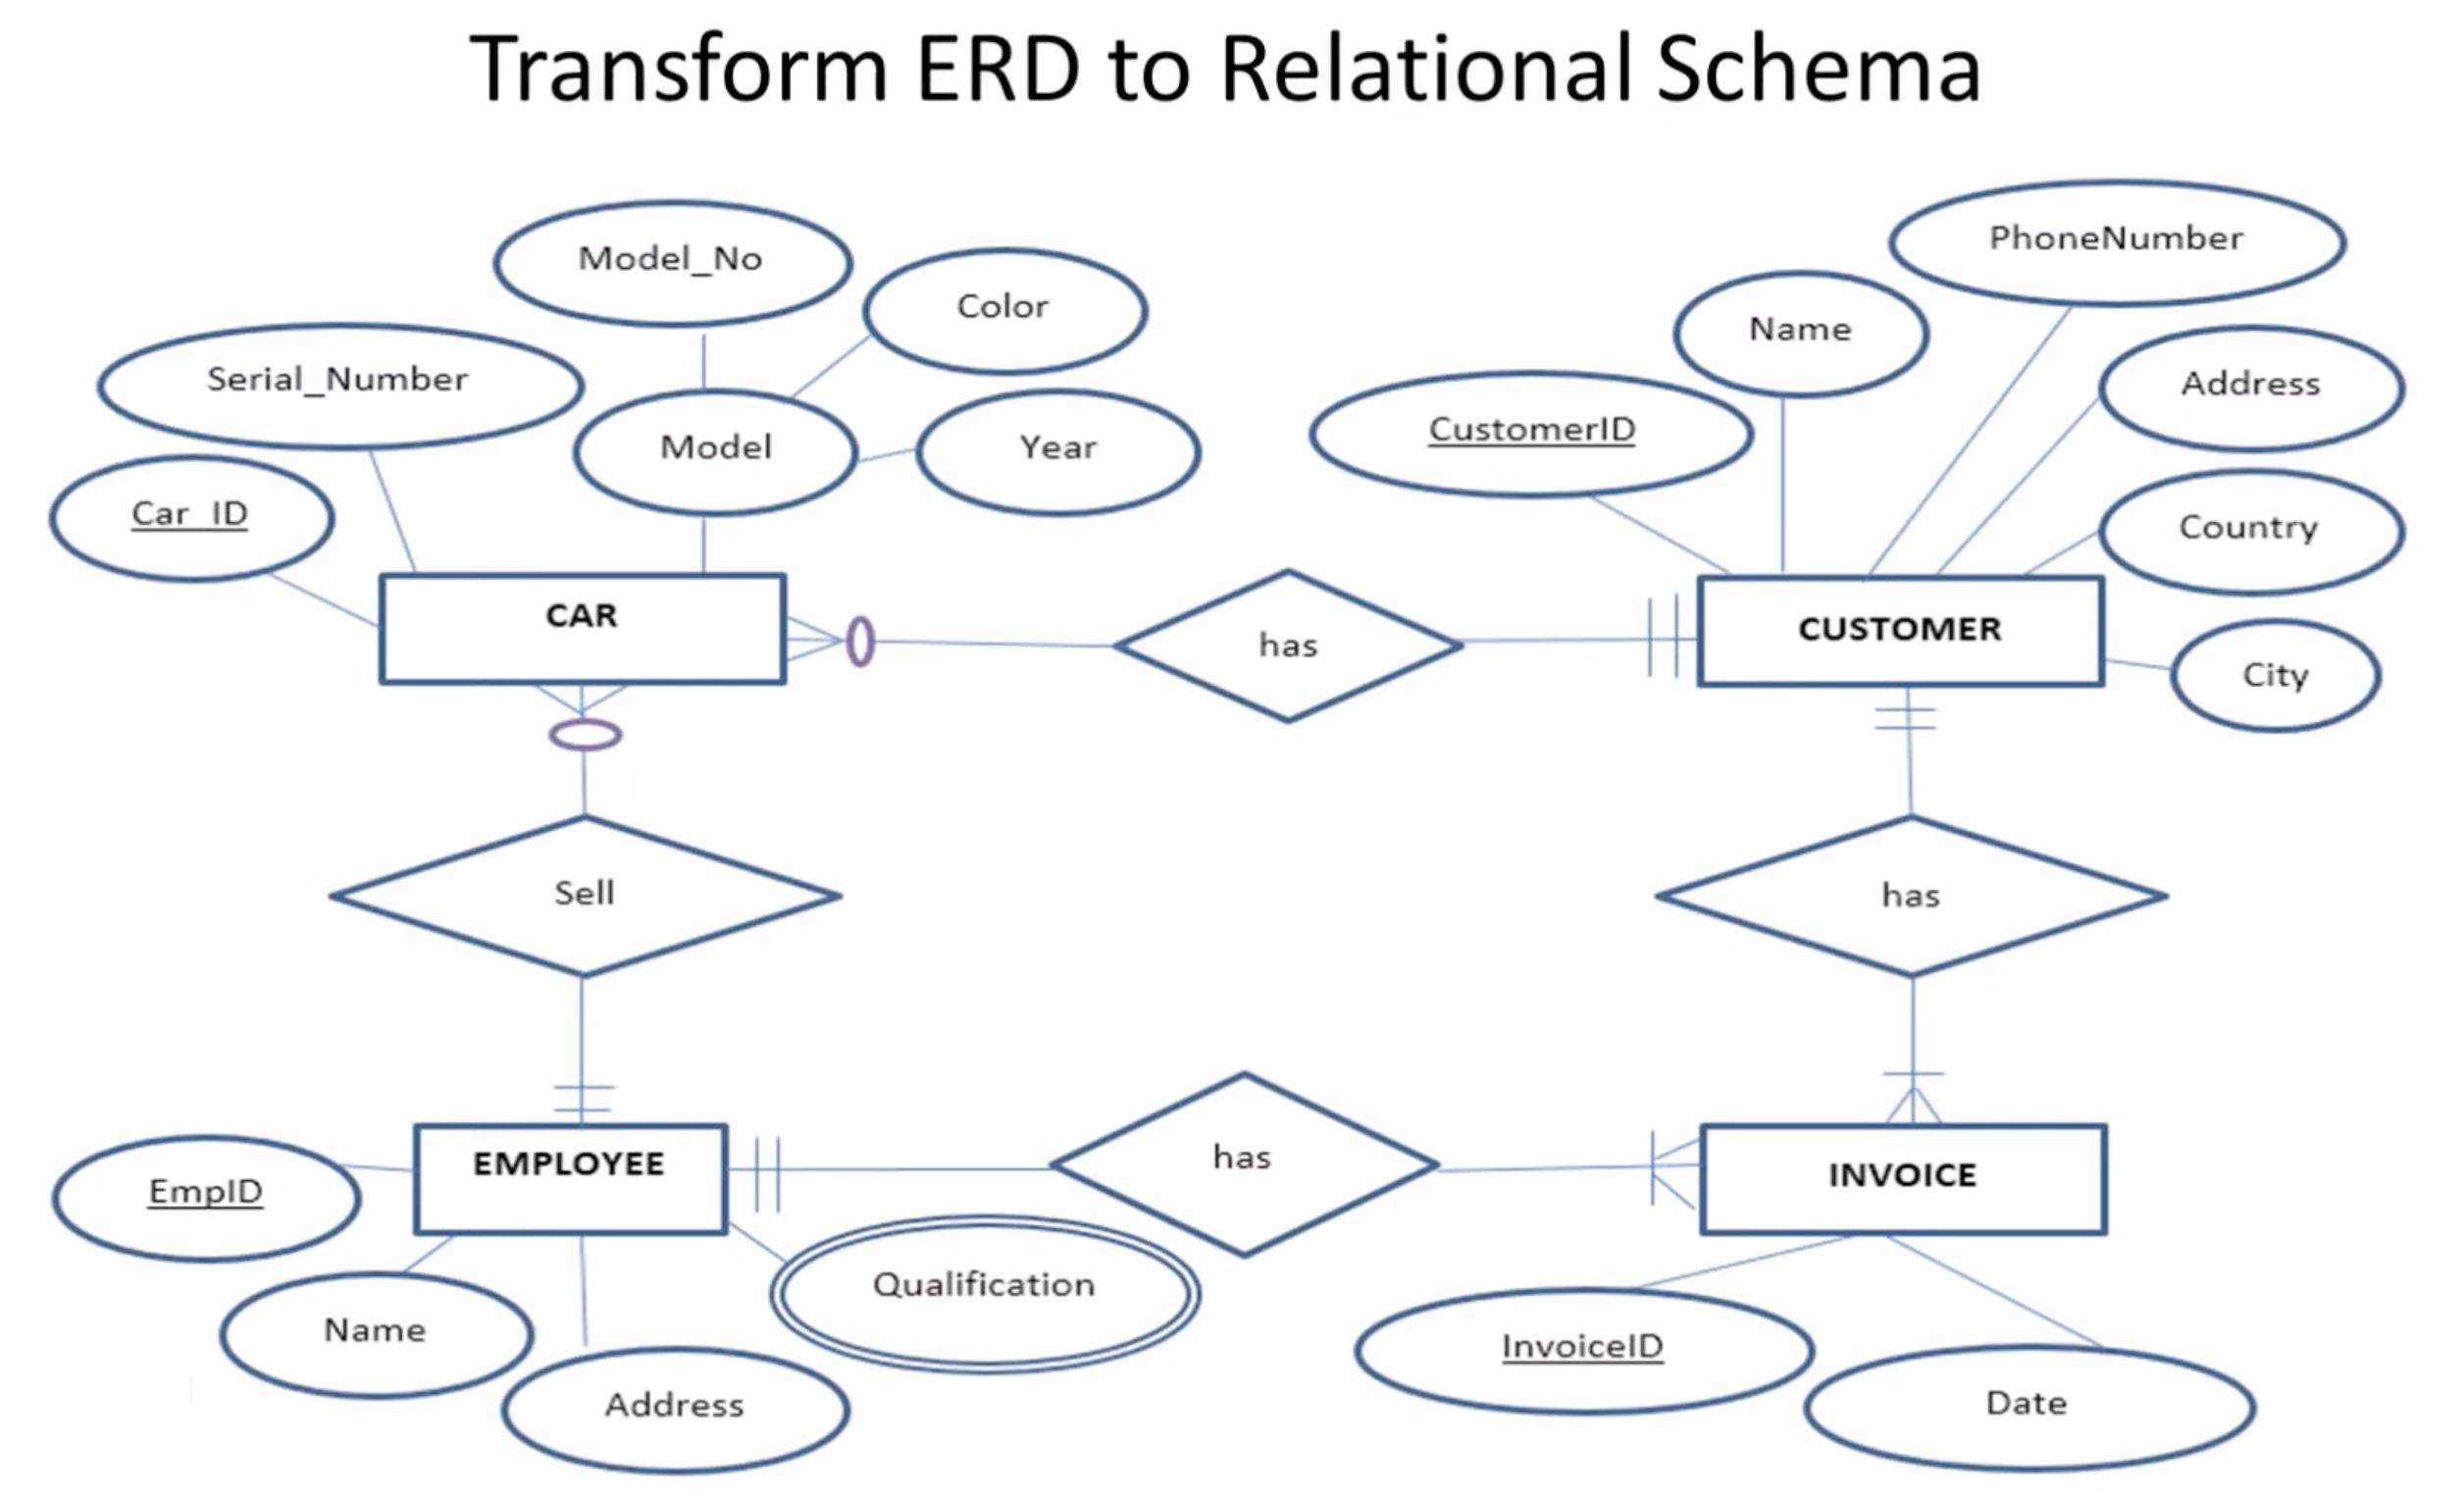
\includegraphics[width=8cm,height=4cm]{logical_model/entity_relation_img}
\end{center}

\vspace{-0.1cm}

\begin{itemize}[noitemsep,leftmargin=*]
\leftskip-\dimexpr\leftmargin %%%
    \item[] \textbf{CAR} table with primary key \textit{Car\_ID}.
    \item[] \textbf{CUSTOMER} table with primary key \textit{CustomerID}.
    \item[] \textbf{EMPLOYEE} table with primary key \textit{EmpID}.
    \item[] \textbf{INVOICE} table with primary key \textit{InvoiceID}, including foreign key \textit{CustomerID}.
    \item[] \textbf{SELL} join table to represent the many-to-many relationship between \textbf{CAR} and \textbf{EMPLOYEE}.
\end{itemize}

\noindent
\begin{minipage}[t]{.5\linewidth}
    \centering
    \begin{tabular}{ll}
        \toprule
        \textbf{CAR} & \\
        \midrule
        Car\_ID & Primary Key \\
        Serial\_Number & \\
        Model & \\
        Model\_No & \\
        Color & \\
        Year & \\
        \bottomrule
    \end{tabular}
\end{minipage}%
\begin{minipage}[t]{.5\linewidth}
    \centering
    \begin{tabular}{ll}
        \toprule
        \textbf{CUSTOMER} & \\
        \midrule
        CustomerID & Primary Key \\
        Name & \\
        PhoneNumber & \\
        Address & \\
        Country & \\
        City & \\
        \bottomrule
    \end{tabular}
\end{minipage}


\noindent
\begin{minipage}[t]{.5\linewidth}
    \centering
    \begin{tabular}{ll}
        \toprule
        \textbf{EMPLOYEE} & \\
        \midrule
        EmpID & Primary Key \\
        Name & \\
        Address & \\
        Qualification & \\
        \bottomrule
    \end{tabular}
\end{minipage}%
\begin{minipage}[t]{.5\linewidth}
    \centering
    \begin{tabular}{ll}
        \toprule
        \textbf{INVOICE} & \\
        \midrule
        InvoiceID & Primary Key \\
        Date & \\
        CustomerID & Foreign Key \\
        \bottomrule
    \end{tabular}
\end{minipage}%

% SELL Join Table
\begin{table}[h!]
    \centering
    \begin{tabular}{ll}
        \toprule
        \textbf{SELL} & \\
        \midrule
        Car\_ID & Foreign Key (References CAR) \\
        EmpID & Foreign Key (References EMPLOYEE) \\
        Sell\_Details & Additional information about the sale \\
        \bottomrule
    \end{tabular}
\end{table}


\section*{SQL}

\subsection*{Keywords}

\begin{itemize}[noitemsep,leftmargin=*]
    \leftskip-\dimexpr\leftmargin %%% 
    \item[]{\textbf{SELECT}: Retrieves data from a database.}
    \item[]{\textbf{FROM}: Specifies the table from where data is retrieved.}
    \item[]{\textbf{WHERE}: Filters records based on specified conditions.}
    \item[]{\textbf{JOIN}: Combines rows from two or more tables based on a related column.}
    \item[]{\textbf{LEFT JOIN}: Returns all records from the left table, and matched records from the right table.}
    \item[]{\textbf{RIGHT JOIN}: Returns all records from the right table, and the matched records from the left table.}
    \item[]{\textbf{NATURAL JOIN}: Performs a join between two tables using all columns with the same names.}
    \item[]{\textbf{INNER JOIN}: Returns rows when there is at least one match in both tables.}
    \item[]{\textbf{GROUP BY}: Arranges identical data into groups.}
    \item[]{\textbf{ORDER BY}: Sorts the result-set in ascending or descending order.}
    \item[]{\textbf{HAVING}: Filters records on aggregated results.}
    \item[]{\textbf{ROUND()}: Rounds a number to a specified number of decimal places - similar to COUNT().}
    \item[]{\textbf{AVG()}: Calculates the average value of a numeric column.}
    \item[]{\textbf{EXPLAIN}: Provides information about how MySQL executes a query.}
    \item[]{\textbf{CREATE INDEX}: Creates an index on a table to improve query performance.}
    \item[]{\textbf{LIKE}: Operator used in a WHERE clause to search for a specified pattern in a column.}
    \item[]{\textbf{AND}: Combines two or more conditions in a WHERE clause.}
    \item[]{\textbf{OR}: Allows for multiple conditions in a WHERE clause, where if any condition is true, the row is included.}
    \item[]{\textbf{ASC}: Specifies ascending order in an ORDER BY clause.}
    \item[]{\textbf{DESC}: Specifies descending order in an ORDER BY clause.}
    \item[]{\textbf{IS NOT NULL}: Operator used in a WHERE clause to filter out rows where specified column's value is not NULL.}
    \item[]{\textbf{\%}: Wildcard character used with LIKE operator to match any sequence of characters.}
    \item[]{\textbf{PRIMARY KEY}: Constraint used to uniquely identify each row in a table.}
    \item[]{\textbf{FOREIGN KEY}: Constraint used to link two tables together.}
\end{itemize}

\begin{lstlisting}[language=SQL]
SELECT 
    b.title AS BookTitle, 
    CONCAT(a.first_name, ' ', a.last_name) AS AuthorName, 
    ROUND(AVG(s.sale_amount)) AS AverageSales,
    COUNT(s.sale_id) AS TotalSales
FROM 
    books b
INNER JOIN authors a ON b.author_id = a.author_id
LEFT JOIN sales s ON b.book_id = s.book_id
WHERE 
    a.last_name LIKE 'R\%' AND
    b.publication_year > 2000 AND
    s.sale_id IS NOT NULL
GROUP BY 
    b.book_id
HAVING 
    COUNT(s.sale_id) > 50
ORDER BY 
    TotalSales DESC, 
    b.title ASC;
\end{lstlisting}

\begin{itemize}[noitemsep,leftmargin=*]
\leftskip-\dimexpr\leftmargin %%% 
\item[]{\textbf{SELECT}: Starts the selection of data.}
\item[]{\textbf{CONCAT()}: Concatenates the author's first and last name.}
\item[]{\textbf{ROUND()}: Rounds the average sales amount to the nearest integer.}
\item[]{\textbf{FROM}: Indicates the books table as the source.}
\item[]{\textbf{INNER JOIN}: Joins the books with the authors where the author\_id matches.}
\item[]{\textbf{LEFT JOIN}: Joins the books with the sales to include all books, even if there are no sales records.}
\item[]{\textbf{WHERE}: Filters the result to authors with a last name starting with 'R' and books published after 2000.}
\item[]{\textbf{LIKE 'R\%'}: Searches for authors with last names beginning with 'R'.}
\item[]{\textbf{AND}: Combines multiple conditions in the WHERE clause.}
\item[]{\textbf{GROUP BY}: Groups the result by book ID to calculate averages and counts per book.}
\item[]{\textbf{HAVING}: Filters groups to include only those with more than 50 sales.}
\item[]{\textbf{ORDER BY}: Orders the results first by TotalSales in descending order, then by BookTitle in ascending order.}
\item[]{\textbf{ASC/DESC}: Specifies the order direction.}
\item[]{\textbf{IS NOT NULL}: Ensures that only sales with valid sale IDs are included.}
\end{itemize}

\subsection*{Data Types}

\begin{itemize}[noitemsep,leftmargin=*]
\leftskip-\dimexpr\leftmargin %%% 
    \item[]{\textbf{INT}: A normal-size integer that can be signed or unsigned.}
    \item[]{\textbf{VARCHAR(n)}: A variable-length string with a maximum length of `n` characters.}
    \item[]{\textbf{TEXT}: A text column with a maximum length of 65,535 characters.}
    \item[]{\textbf{DATE}: A date, formatted as YYYY-MM-DD.}
    \item[]{\textbf{TIMESTAMP}: A timestamp, combining a date and a time.}
    \item[]{\textbf{FLOAT(p, d)}: A floating-point number with a precision `p` and a scale `d`.}
    \item[]{\textbf{DOUBLE(p, d)}: A double precision floating-point number.}
    \item[]{\textbf{DECIMAL(p, d)}: An exact fixed-point number.}
    \item[]{\textbf{BOOLEAN}: A true or false value.}
    \item[]{\textbf{BLOB}: A binary large object that can hold a variable amount of data.}
    \item[]{\textbf{CHAR(n)}: A fixed-length non-binary string.}
    \item[]{\textbf{BIGINT}: A large integer that can be signed or unsigned.}
    \item[]{\textbf{ENUM(val1, val2, ...)}: A string object that can only have one value, chosen from a list of possible values.}
    \item[]{\textbf{SET(val1, val2, ...)}: A string object that can have zero or more values, chosen from a list of possible values.}
\end{itemize}


\vspace{-0.1cm}
\subsection*{Disk Storage}
\vspace{-0.1cm}

\noindent
Physically stored on magnetic or solid-state disks.

\begin{itemize}[noitemsep,leftmargin=*]
\leftskip-\dimexpr\leftmargin %%%
\item[]{\textbf{Data Blocks}: The smallest unit of data storage on a disk. Databases often read or write one block at a time.}
\item[]{\textbf{Sectors and Tracks}: Physical divisions of a disk; sectors are subdivisions of tracks.}
\item[]{\textbf{File Organization}: How records are physically arranged on a disk - sequential, direct, or indexed.}
\item[]{\textbf{Partitions}: Division of a database table into smaller parts for performance and manageability.}
\item[]{\textbf{Physical Design}: Involves the design of physical storage, file organization, and indexing for performance optimization.}
\end{itemize}

\vspace{-0.3cm}
\subsection*{File Structure}
\vspace{-0.1cm}

\begin{itemize}[noitemsep,leftmargin=*] 
\leftskip-\dimexpr\leftmargin %%%
\item[]{\textbf{Sequential}: Records are stored in sequential order, typically sorted by a key field.}
\item[]{\textbf{Direct or Hashed}: Records are stored in seemingly random order but according to a calculated position (hash).}
\item[]{\textbf{Indexed}: Uses indexes to quickly locate data without scanning the entire file.}
\end{itemize}

\vspace{-0.3cm}
\subsection*{Indexing}
\vspace{-0.1cm}

\noindent
Used to speed up the retrieval of data.

\begin{itemize}[noitemsep,leftmargin=*] 
\leftskip-\dimexpr\leftmargin %%%
\item[]{\textbf{Primary/Secondary Index:} Primary index uses the unique table identifier, while secondary index uses non-primary fields for data access.}
\item[]{\textbf{Index:} A data structure that allows for faster data retrieval from a database.}
\item[]{\textbf{Index File:} A separate file containing indexes to improve data search efficiency in database tables.}
\item[]{\textbf{Sparse Indices:} Index type with entries for some records, requiring less space but potentially slower navigation.}
\item[]{\textbf{Dense Indices:} Index type with an entry for every record, providing faster lookup at the expense of more space.}
\end{itemize}

\vspace{-0.3cm}
\subsection*{Transactions}
\vspace{-0.1cm}

\begin{itemize}[noitemsep,leftmargin=*]
\leftskip-\dimexpr\leftmargin %%%
\item[]{\textbf{Deadlock:} A situation in concurrent transactions where transactions wait indefinitely for each other's resources.}
\item[]{\textbf{Atomicity:} A property ensuring all operations in a transaction are completed successfully or not at all.}
\item[]{\textbf{Consistency:} Ensures a transaction transitions the database from one valid state to another, maintaining data integrity.}
\item[]{\textbf{Isolation:} The property that defines the visibility of transaction changes to other transactions.}
\item[]{\textbf{Durability:} Ensures that once a transaction is committed, it remains so even after a system failure.}
\item[]{\textbf{ACID}: Atomicity, Consistency, Isolation, Durability}
\item[]{\textbf{Isolation Levels:} Defines the degree of isolation between transactions, impacting concurrency and consistency.}
\end{itemize}




\end{document}